\documentclass[11pt,letterpaper]{article}

%\usepackage{fontspec}
%\usepackage[utf8]{inputenc}
\usepackage{textcomp,marvosym}
\usepackage{amsmath,amssymb}
\usepackage[normalem]{ulem}
\usepackage[left]{lineno}
\usepackage{booktabs}
\usepackage{changepage}
\usepackage{rotating}
\usepackage{color}
\usepackage{natbib}
\usepackage{setspace}
\usepackage{array}
\usepackage{fancyhdr}
\usepackage{graphicx}
\usepackage{xspace}
\usepackage[hidelinks]{hyperref}
\urlstyle{same}
\usepackage{threeparttable}
\doublespacing

\raggedright
\textwidth = 6.5 in
\textheight = 8.25 in
\oddsidemargin = 0.0 in
\evensidemargin = 0.0 in
\topmargin = 0.0 in
\headheight = 0.0 in
\headsep = 0.5 in
\parskip = 0.1 in
\parindent = 0.2in

% Bold the 'Figure #' in the caption and separate it from the title/caption with a period
% Captions will be left justified
\usepackage[aboveskip=1pt,labelfont=bf,labelsep=period,justification=raggedright,singlelinecheck=off]{caption}

% Remove brackets from numbering in List of References
%\makeatletter
%\renewcommand{\@biblabel}[1]{\quad#1.}
%\makeatother

% Self defined commands
\newcommand{\degC}{$^{\circ}$C\xspace}
\newcommand{\dC}{$\delta^{13}$C\xspace}
\newcommand{\dO}{$\delta^{18}$O\xspace}
\newcommand{\SrSr}{$^{87}$Sr/$^{86}$Sr\xspace}
\newcommand{\permil}{\textperthousand\xspace}
\newcommand{\dsil}{$d$\xspace}
\newcommand{\UPb}{$^{206}$Pb/$^{238}$U\xspace}
%

\pagestyle{myheadings}
\pagestyle{fancy}
\fancyhf{}
\lhead{Park et al., in preparation for AGU book entitled \textit{Environmental Change and Large Igneous Provinces}}
\rhead{\thepage}

\begin{document}

\begin{flushleft}
{\Large \textbf{Evaluating the relationship between the area and latitude of large igneous provinces and Earth's long-term climate state}}

Yuem Park\textsuperscript{1},
Nicholas L. Swanson-Hysell\textsuperscript{1},
Lorraine E. Lisiecki\textsuperscript{2},
Francis A. Macdonald\textsuperscript{2}

\bigskip
\textsuperscript{1} Department of Earth and Planetary Science, University of California, Berkeley, CA, USA

\textsuperscript{2} Department of Earth Science, University of California, Santa Barbara, CA, USA
\bigskip

\end{flushleft}

\noindent\textit{This article is in preparation for submission to the AGU book \textit{Environmental Change and Large Igneous Provinces}.}

\linenumbers

\section*{ABSTRACT \label{sec:ABSTRACT}}

One of the hypothesized effects of the emplacement of large igneous provinces (LIPs) is planetary cooling on million-year timescales associated with enhanced silicate weathering. A systematic analysis of LIP area and latitude through the Phanerozoic reveals that there is no significant correlation between total LIP area, nor LIP area in the tropics, and the extent of continental ice sheets. The largest peaks in tropical LIP area are at times of non-glacial climate. These results suggest that changes in planetary weatherability associated with LIPs are not the fundamental control on whether Earth is in a glacial or non-glacial climate, although they could provide a secondary modulating effect in conjunction with other processes.

\section*{INTRODUCTION \label{sec:INTRODUCTION}}

Global weatherability is the sum of factors aside from climate itself, such as the latitudinal distribution of continents and mountain belts, that contribute to overall global weathering and associated CO$_2$ consumption. On a planet with high weatherability, the CO$_2$ input from volcanism can be removed via silicate weathering at a lower atmospheric CO$_2$ concentration than on a less weatherable planet. Basaltic regions consume more CO$_2$ than regions where bedrock composition is closer to bulk continental crust because of the relatively high concentrations of Ca and Mg (that ultimately sequester carbon through precipitation as carbonate) and the high weathering rates of mafic lithologies \citep{Dessert2003a}. Data from basaltic watersheds show that chemical weathering rates are greatest in regions with high runoff, and as a result CO$_2$ consumption in basaltic regions is most pronounced in the tropical rain belt \citep{Dessert2003a, Hartmann2009a, Hartmann2014a}.

One aspect of large igneous province (LIP) emplacement that has been hypothesized to relate to long-term global climate is the effect such emplacement could have on increasing global weatherability and driving cooling. In particular, the emplacement of LIPs in the tropics has been hypothesized to be associated with specific episodes of climatic cooling on Earth. In the Neoproterozoic Era, the emplacement of the ca. 720~Ma Franklin LIP in the tropics, in concert with elevated runoff rates associated with continental break-up, has been implicated as a major contributor to the cooling that initiated the Sturtian `Snowball Earth' \citep{Donnadieu2004b, Macdonald2010a, Cox2016a}. In the Cenozoic, the movement of the Deccan LIP into the tropical rain belt, in concert with the low-latitude emplacement of the Ethiopian Traps, has been implicated in drawing down CO$_2$ levels in the lead-up to Oligocene glaciation of Antarctica \citep{Kent2008a, Kent2013a}.

This chapter seeks to address two interconnected questions: 1) how unique are the peaks in low-latitude LIP area that have been proposed to be associated with climatic cooling?; and 2) how strong is the overall relationship between tropical LIP area and glaciation?

\section*{METHODS}

Outlines of the original surface extent of LIPs through the Phanerozoic (Fig. \ref{fig:LIP_map}) were slightly modified from the compilation of \citet{Ernst2017a}, and emplacement ages were taken from the literature (Table \ref{tab:LIPs}). The compilation of \citet{Ernst2017a} seeks to reconstruct the original surface extent of LIPs with the caveat that there can be significant uncertainty with doing so, particularly for older more deeply eroded LIPs. These polygons encapsulate all of the rocks associated with a given LIP, including dikes, sills, and layered intrusions in addition to subaerial volcanics (Fig. \ref{fig:LIP_map}). For some LIPs, this approach may lead to an overestimate of original surface extent, given that subsurface intrusions could extend over a broader area than the surface volcanics. The polygons also assume complete surface coverage between wide-spread remnants, creating further potential for these outlines being over-estimates. However, this approach likely provides the best estimates available of original extent for ancient LIPs. The extents of presently-exposed volcanics associated with LIPs that were used for present-day area estimates, and the construction of the original extent polygons by \citet{Ernst2017a}, were taken from a number of resources including the PLATES compilation \citep{Coffin2006a} and more recent compilation efforts associated with the LIPs Reconstruction Project (\citealp{Ernst2013a}; Table \ref{tab:LIPs}).

After LIPs are emplaced, they will progressively erode. In order to account for this decrease in area with time, \citet{Godderis2017a} took the approach of fitting an exponential decay function to estimates of the original surface extent and the current surface extent for 5 LIPs. They used the resulting exponential decay constants to develop a first-order model to estimate changing LIP area through time. We extend this approach to 19 basaltic LIPs for which we have estimates of the original surface extent of the province and the current surface extent of rocks associated with it (Fig. \ref{fig:LIP_preservation}). While there are significant uncertainties associated with the area estimates, this compilation suggests that an exponential decay function is an appropriate first-order model for the progressive reduction in LIP area. The best-fit exponential function results in a LIP area half-life of 29~Myr. However, since we explicitly account for LIP burial separately in our models (see below), we prefer to exclude from our estimation of a representative LIP area half-life the 6 of 19 LIPs which have been partially or completely buried. This latter approach yields a slightly higher best-fit half-life of 36~Myr (Fig. \ref{fig:LIP_preservation}). Although the root mean square error of the fit is low (0.14), there is variability in the half-lives for LIPs if they are fit individually with an exponential decay function, such that they range from shorter half-lives of $\sim$20~Myr up to $\sim$120~Myr for the Kalkarindji and Deccan Traps (Table \ref{tab:LIPs}). In the analysis of LIP area through time, we implement decay scenarios informed by this analysis. Scenario `t$_{1/2}$ = 36~Myr' uses the best-fit half-life of 36~Myr, while `t$_{1/2}$ = 120~Myr' uses the slower decay. Given that the post-emplacement weathering and erosional history of each LIP should be dependent on the tectonic and climatic setting that each LIP experiences during and after emplacement, this approach is simplistic but provides a framework for analysis. The LIP reconstructions used in this study also include pre-Phanerozoic LIPs. However, given the imposed exponential decay since emplacement, the inclusion of these LIPs does not significantly impact the calculated LIP areas throughout the Phanerozoic, which is the focus of this analysis.

Of the tectonic factors that could alter exposed LIP area, the most consequential is near-immediate burial by sediments of LIP volcanics that are co-located with a rift basin. There are numerous examples in the record where there is partial or complete burial of a LIP associated with rifting and thermal subsidence (Table \ref{tab:LIPs}). For example, the Afar LIP is both associated with the Ethiopian Traps which form plateau flood basalts as well as successful rifting in the region of the Red Sea that has resulted in burial (Fig. \ref{fig:LIP_map}). To account for the rapid decrease in exposed surface area that would result from burial by sediments in a rift basin, we impose two different burial scenarios for LIPs that are co-located with rifting. The `50\% burial' scenario imposes instantaneous burial of 50$\%$ of the LIP area while the `100\% burial' imposes instantaneous burial of the entire LIP as an end-member scenario. The LIP area analysis uses all of the available combinations of these distinct decay and burial scenarios.

Our LIP reconstruction differs from that of \citet{Johansson2018a} in several respects. In contrast to the decay and decay+burial scenarios implemented on estimates of original LIP extent in this study, \citet{Johansson2018a} uses a static extent for each LIP throughout the reconstruction with some of the polygons corresponding to the present-day surface extent and some representing the original extent that includes currently buried portions of the LIP (e.g. the Keweenawan Midcontinent Rift for which the implemented extent is from geophysical data that largely correponds to buried subsurface exposures).

The original extent LIP polygons were assigned a plate ID corresponding to a tectonic unit on Earth using the polygons of \citet{Torsvik2016a} for the Phanerozoic. The LIP polygons and tectonic units were reconstructed from 520~Ma to the present utilizing the paleogeographic model of \citet{Torsvik2016a} in the spin axis reference frame (anchor plate ID of 1). This paleogeographic model was updated to include a revision to Ordovician Laurentia \citep{Swanson-Hysell2017a} and Paleozoic Asia \citep{Domeier2018a}. Reconstructions and area calculations within latitude bands utilized the pyGPlates function library and custom Python scripts documented within a Jupyter notebook that reproduces the analysis and development of the associated visualizations. The total LIP area and the LIP area reconstructed within the tropical rain belt (15\textdegree~S to 15\textdegree~N) were calculated for the various decay and burial scenarios at a resolution of 5~Myr (Fig. \ref{fig:LIP_area}B and C). We use 15\textdegree~S to 15\textdegree~N as the definition of the tropical rain belt, as those latitudes approximately correspond with precipitation greater than 1.0~m/yr in modern climatalogical data \citep{Kalnay1996a}. The consistent paleolatitudes of evaporite deposits in the subtropics demonstrate the stability of the large-scale atmospheric circulation that gives rise to intense precipitation in the tropical rain belt \citep{Evans2006a}.

To evaluate the relationship between Earth's climate state and tropical LIP area, we compared these areas to a compilation of the latitudinal extent of continental ice sheets through time over the Phanerozoic (\citealp{Macdonald2018a}; Fig. \ref{fig:LIP_area}E). The goal in doing so is to evaluate the hypothesis that there is a correlation between LIP area in the tropics and Earth's long-term climate state. The land ice record is an imperfect tracker of climate, as it is insensitive to changes in temperature during non-glacial intervals and is influenced by additional factors such as the physical geography of the continents during glacial intervals. Nevertheless, it forms a physical record of Earth's climate through time and delineates glacial and non-glacial climate states. We take two approaches for comparison between the LIP area reconstruction and the record of ice extent. The first is to analyze the correlation between LIP area and the extent of ice away from the pole (Fig. \ref{fig:LIP_correlation}). The second is to consider the overlap between intervals of high LIP area (defined as LIP area \textgreater30\% of the maximum in a given post-emplacement model) and intervals of glacial climate (defined as ice extent \textgreater10\textdegree\xspace from the poles). This overlap approach places less emphasis on the specific magnitudes of the compiled ice extent and LIP area records.

Another approach would be to compare LIP area records to proxy compilations of \textit{p}CO$_2$ (as done by \citealp{Johansson2018a}). However, such proxy compilations are problematic as they are poorly calibrated in deep time, prone to alteration, and reliant on a myriad of assumptions. We thus prefer to use the latitudinal extent of land ice to reflect Earth's overall climate state throughout the Phanerozoic.

\section*{RESULTS}

In the `t$_{1/2}$ = 36~Myr' scenario, we observe three primary peaks and one minor peak in the calculated LIP area within the tropics (Fig. \ref{fig:LIP_area}C). The first primary peak ca. 510~Ma is associated with the emplacement of the Kalkarindji LIP, the second primary peak ca. 380~Ma is associated with the emplacement of the Kola-Dnieper LIP, the third primary peak ca. 200~Ma is associated with the emplacement of the CAMP, and the minor Cenozoic peak is associated with both the ca. 30~Ma emplacement of the Afar LIP as well as the earlier drift of the ca. 66~Ma Deccan LIP into the tropics (Fig. \ref{fig:LIP_area}A). When we account for burial (`t$_{1/2}$ = 36~Myr + 50\% burial' and `t$_{1/2}$ = 36~Myr + 100\% burial' scenarios), only the latter two of these four peaks are affected -- the ca. 200~Ma peak is attenuated/removed due to the partial/complete burial of the CAMP, and the Cenozoic peak is attenuated due to the partial/complete removal of the Afar LIP. However, after accounting for burial, a minor area of LIPs remain in the tropics from ca. 130~Ma onwards, due to the EQUAMP, Caribbean-Colombian, and Deccan LIPs. Using the longer decay half-life of 120~Myr (the `t$_{1/2}$ = 120~Myr + 100\% burial' scenario) increases the area of LIPs in the tropics at any given time step, and has the effect of extending the duration of each peak.

The only scenario which results in a positive Pearson correlation coefficient (0.10) between LIP area in the tropics (Fig. \ref{fig:LIP_area}C) and the ice extent record (Fig. \ref{fig:LIP_area}E) is the scenario with the slow decay rate and complete burial of LIPs associated with rifting (the `t$_{1/2}$ = 120~Myr + 100\% burial' scenario; Fig. \ref{fig:LIP_correlation}). All other scenarios yield a near zero or weak negative correlation coefficient. Qualitatively, the weak positive correlation of the `t$_{1/2}$ = 120~Myr + 100\% burial' scenario relative to the other scenarios can be primarily attributed to the complete removal of the CAMP, which was emplaced during an extended interval of ice-free conditions, as well as the effect of the longer decay half-life extending the duration of the earlier two peaks, such that they overlap more with the Late Ordovician and Permo-Carboniferous glacial intervals.

To assess the statistical significance of the correlation (or lack thereof) implied by the Pearson correlation coefficients, we simulated the four glacial episodes (Fig. \ref{fig:LIP_area}E) occurring at random times through the past 520~Myr, and recomputed the correlation coefficient and \% overlap between the LIP area in the tropics and the randomly timed glacial intervals for each of these 100,000 simulations (Fig. \ref{fig:LIP_correlation}). This approach accounts for the reality that spurious correlation can arise between auto-correlated data sets such as these, where each value is not independent, but is instead dependent on the previous state of the system. For the `t$_{1/2}$ = 120~Myr + 100\% burial' scenario, 28\% of the randomly timed glacial intervals correlate better with the LIP area in the tropics. With an associated p-value of 0.28, the null hypothesis that glacial intervals do not correlate to LIP area in the tropics cannot be rejected. Taking this approach, none of the positive or negative correlations that emerge between the LIP area scenarios are statistically significant.

\section*{DISCUSSION}

The results from this analysis indicate that when the entire LIP database is considered, there is no significant relationship between total LIP area or LIP area in the tropics and the extent of continental ice sheets (Fig. \ref{fig:LIP_correlation}). While this result need not imply that there is no increase in global weatherability from the emplacement of LIPs, it does suggest that LIP area is not the fundamental control on Earth's long-term climate state.

In the original models that proposed the `Fire and Ice' hypothesis as an explanation for the onset of the Sturtian `Snowball Earth' glaciation, chemical weathering was modeled as an Arrhenius relationship where it was solely a function of temperature and run-off \citep{Donnadieu2004a}. However, such an approach neglects the effects of soil shielding and regolith development in low-relief regions. Recent progress on understanding the relationships between landscapes, topography, and chemical weathering reveals that these effects are quite important \citep{Gabet2009a, Maher2014a}. As a result, more recent modeling of chemical weathering that has incorporated such processes highlights the importance of high-relief regions relative to low-relief ones \citep{Godderis2017b}. Without active uplift, soil shielding from regolith development on low-relief LIPs could significantly decrease the local weatherability of a LIP and mute its impact on global weatherability. In contrast, processes that lead to continued exhumation of mafic lithologies and the creation of steep topography, particularly in tropical regions, may exert a strong control on global weatherability and long-term climate. This interpretation underlies the hypothesis that arc-continent collisions in the tropics during the Ordovician \citep{Swanson-Hysell2017a} and the Cenozoic \citep{Jagoutz2016a} played a significant role in transitions into glacial climate states at those times.

A complication with the interpretation of soil shielding and limited weathering of LIPs is the rapid area decay rate inferred from the comparison of current LIP extent to estimated original extent (Fig. \ref{fig:LIP_preservation}). A couple considerations are relevant with respect to this analysis: 1) the current extent of LIP exposure is reduced in part by volcanics being covered by unconsolidated sediments (i.e. regolith development itself) in a number of the provinces; 2) the current extent of LIP exposure may be incomplete and an underestimate for some of the provinces; 3) the initial LIP extents are typically poorly constrained and are likely overestimates which could be resulting in inflated interpreted decay rates; and 4) the relationship between LIP area and volume is poorly constrained. Future efforts that improve the LIP database, such as developing better-constrained estimates of original LIP extent, constraining burial and uplift histories, and refining the timing of eruptions associated with LIPs, will improve analyses such as that in this contribution.

We have focused this analysis on the Phanerozoic record given that well-constrained paleogeographic models are available for the past $\sim$520~Myr. Furthermore, the approach of seeking to evaluate correlation between LIP area and glaciation is complicated for Neoproterozoic Snowball Earth events, since ice-albedo runaway leads to persistent global glaciation absent of continued forcing through normal carbon cycle processes until sufficient CO$_2$ builds up in the absence of silicate weathering to drive deglaciation. Nevertheless, the hypothesis of tropical LIP area associated with the ca. 720~Ma Franklin LIP increasing global weatherability and contributing to the onset of the Sturtian Snowball Earth is a major motivating driver behind conducting this analysis. How does the tropical LIP area associated with the Franklin LIP compare to that observed in the Phanerozoic? Using the paleomagnetic pole of \citet{Denyszyn2009a}, we reconstruct the paleolatitude of the Franklin LIP at the time of emplacement, and find that $\sim$99.7\% (or $\sim$2.6~Mkm$^{2}$) of the LIP erupted within 15\textdegree\xspace of the equator. This Franklin LIP tropical area at the time of emplacement is approximately equivalent to the Cenozoic peak, and is smaller than the other Phanerozoic peaks (Fig. \ref{fig:LIP_area}C). The ca. 1109~Ma Umkondo is another Precambrian LIP that is constrained to have erupted in the tropics, although it is not known to be associated with any glaciation (no glacial deposits are found within the contemporaneous Midcontinent Rift basin; \citealp{Swanson-Hysell2018a}). We reconstruct the paleolatitude of the Umkondo LIP at the time of emplacement using the paleomagnetic pole of \citet{Swanson-Hysell2015b}, and find that effectively all of the LIP (or $\sim$2.0~Mkm$^{2}$) erupted within the tropics, an area that is slightly smaller than that for the Franklin LIP (Fig. \ref{fig:LIP_area}C). Together, these results indicate that the tropical area of the Franklin LIP, when compared to that of Phanerozoic as well as other Precambrian LIPs, did not have a singularly large area in the tropics. Given that similar peaks in tropical LIP area are not associated with the onset of glacial periods, additional processes must have been at play in drawing down atmospheric CO$_2$ in the lead-up to the Sturtian Snowball Earth. One such process could have been an increase in global weatherability associated with arc accretion within terranes of the present-day Arabian-Nubian Shield \citep{Park2018a}. An increase in global weatherability associated with the emplacement of the Franklin LIP in the tropics could have been a contributing factor in addition to other such processes. The temporal overlap between Franklin LIP eruptions \citep{Denyszyn2009a} and the initiation of Sturtian glaciation \citep{Macdonald2010a, MacLennan2018a} remains compelling. This overlap continues to suggest that other aspects of LIP emplacement, such as the injection of sulfur aerosols in the stratosphere \citep{Macdonald2017a}, could have played a role in the initiation of low-latitude glaciation. The latitude of such aerosol injections is important for their temporary effect on albedo which is maximized at low latitude, and their presence at high concentrations is pre-conditioned on eruption through sedimentary basins hosting evaporite deposits \citep{Macdonald2017a}. Overall, the conclusion that tropical LIP area associated with the Franklin is not uniquely high and therefore not a sole driver of Snowball Earth onset is consistent with the results of the Phanerozoic analysis. LIP area and its associated impact on global weatherability is not the fundamental control on Earth's long-term climate state.

\section*{ACKNOWLEDGEMENTS \label{sec:ACKNOWLEDGEMENTS}}

Richard Ernst provided GIS compilations of LIP extent and present-day exposure that were essential to the analysis. Discussions with Yves Godd\'eris were valuable in contributing to aspects of the interpretation. Park was supported by NSF Grant 1547434 awarded to Swanson-Hysell.

\clearpage
\newpage

\section*{TABLES}

\begin{table}[h!]
\scriptsize
\caption{Phanerozoic large igneous provinces (and the Franklin).}
\resizebox{\textwidth}{!}{
\begin{tabular}{lc>{\raggedright}p{4cm}cc>{\raggedright}p{4cm}ccl}
\toprule
\textbf{name} & \textbf{age} & \textbf{age ref.} & \textbf{original} & \textbf{present} & \textbf{present area ref.} & \textbf{present/} & \textbf{half-life}$^{1}$ & \textbf{buried?} \\
 & \textbf{(Ma)} & & \textbf{area} & \textbf{area} & & \textbf{original} & \textbf{(Myr)} & \\
 & & & \textbf{(Mkm$^{2}$)} & \textbf{(Mkm$^{2}$)} & & & & \\
\midrule
Columbia River & 16 & \cite{Kasbohm2018a} & 0.68 & 0.38 & \cite{Buchan2004a} & 0.56 & 19.2 & no \\
 & & & & & & & & \\
Afar & 30 & \cite{Courtillot2003a} & 2.05 & 0.63 & \cite{Coffin2006a} & 0.31 & 17.7 & partial \\
 & & & & & & & & \\
NAIP & 62 & \cite{Larsen2015a} & 1.07 & 0.29 & \cite{Buchan2004a, Coffin2006a} & 0.27 & 33.0 & partial \\
 & & & & & & & & \\
Deccan & 66 & \cite{Schoene2014a} & 0.83 & 0.56 & \cite{Coffin2006a} & 0.68 & 116.6 & no \\
 & & & & & & & & \\
Seychelles & 66 & \cite{Schoene2014a} & 0.46 & 0.00 & \cite{Coffin2006a} & 0.00 & 0.0 & yes \\
 & & & & & & & & \\
Madagascar & 90 & \cite{Cucciniello2010a} & 0.63 & 0.03 & \cite{Coffin2006a} & 0.05 & 20.8 & no \\
 & & & & & & & & \\
Caribbean-Colombian & 94 & \cite{Loewen2013a} & 0.71 & 0.13 & \cite{Coffin2006a} & 0.18 & 37.6 & no \\
 & & & & & & & & \\
HALIP & 95 & \cite{Kingsbury2018a} & 3.60 & 0.15 & \cite{Moosdorf2015a} & 0.04 & 20.7 & no \\
 & & & & & & & & \\
EQUAMP & 131 & \cite{Hollanda2016a} & 0.66 & 0.01 & \cite{Hollanda2016a} & 0.01 & 20.5 & no \\
 & & & & & & & & \\
Comei & 132 & \cite{Zhu2009a} & 0.11 & - & - & - & - & no \\
 & & & & & & & & \\
Bunbury & 132 & \cite{Zhu2009a} & 0.03 & 0.00 & \cite{Thorne2014a} & 0.05 & 30.9 & no \\
 & & & & & & & & \\
Parana-Etendeka & 135 & \cite{Florisbal2014a, Almeida2018a} & 3.12 & 0.40 & \cite{Coffin2006a} & 0.13 & 45.7 & partial \\
 & & & & & & & & \\
Trap & 140 & \cite{Ernst2001a} & 0.03 & 0.00 & \cite{Ernst2001a} & 0.00 & 0.0 & no \\
 & & & & & & & & \\
NW Australia Margin & 160 & \cite{Pirajno2012a} & 0.62 & 0.00 & \cite{Coffin2006a} & 0.00 & 0.0 & yes \\
 & & & & & & & & \\
Karoo & 183 & \cite{Burgess2015a} & 3.21 & 0.15 & de Kock compilation$^{2}$ & 0.05 & 41.3 & no \\
 & & & & & & & & \\
Ferrar & 183 & \cite{Burgess2015a} & 0.18 & - & - & - & - & no \\
 & & & & & & & & \\
CAMP & 201 & \cite{Blackburn2013a} & 11.46 & 0.23 & Marzoli and Parisio compilation$^{3}$ & 0.02 & 35.7 & partial \\
 & & & & & & & & \\
Siberia & 252 & \cite{Burgess2015b} & 3.46 & 0.47 & \cite{Coffin2006a} & 0.14 & 87.5 & no \\
 & & & & & & & & \\
Emeishan & 259 & \cite{Zhou2002a} & 0.71 & 0.06 & \cite{Coffin2006a} & 0.09 & 72.9 & no \\
 & & & & & & & & \\
Panjal-Qiangtang & 283 & \cite{Zhai2013a} & 0.11 & - & - & - & - & no \\
 & & & & & & & & \\
Tarim & 290 & \cite{Xu2014a} & 0.35 & - & - & - & - & no \\
 & & & & & & & & \\
Magdalen & 360 & \cite{Brendan_Murphy1999a} & 0.42 & - & - & - & - & no \\
 & & & & & & & & \\
Vilyui & 374 & \cite{Ricci2013a} & 1.14 & - & - & - & - & no \\
 & & & & & & & & \\
Kola-Dnieper & 380 & \cite{Arzamastsev2014a} & 5.90 & - & - & - & - & no \\
 & & & & & & & & \\
Suordakh & 450 & \cite{Khudoley2013a} & 0.02 & - & - & - & - & no \\
 & & & & & & & & \\
Kalkarindji & 511 & \cite{Jourdan2014a} & 3.54 & 0.17 & \cite{Thorne2014a} & 0.05 & 116.3 & no \\
 & & & & & & & & \\
Franklin & 720 & \cite{Denyszyn2009a} & 2.62 & 0.04 & \cite{Buchan2004a} & 0.02 & 121.8 & no \\
\bottomrule
\end{tabular}
}
\begin{tablenotes}[para,flushleft]
$^{1}$assuming exponential decay with form $N(t) = 2^{t/t_{1/2}}$.

$^{2}$from ArcGIS compilation produced by M. de Kock for the LIPs Reconstruction Project \citep{Ernst2013a}.

$^{3}$from ArcGIS compilation produced by A. Marzoli and L. Parisio for the LIPs Reconstruction Project \citep{Ernst2013a}.
\end{tablenotes}
\label{tab:LIPs}
\end{table}

\clearpage
\newpage

\section*{FIGURES}

\begin{figure}[h!]
\begin{center}
	\includegraphics[width=\textwidth]{Manuscript/Figures/LIP_Map.pdf}
	\caption{Map of current extent of volcanic lithologies associated with LIPs that erupted between 520~Ma and the present, as well as the estimates of the initial LIP area used in the area analysis (modified slightly from \citealp{Ernst2017a}).}
	\label{fig:LIP_map}
\end{center}
\end{figure}

\begin{figure}[h!]
\begin{center}
	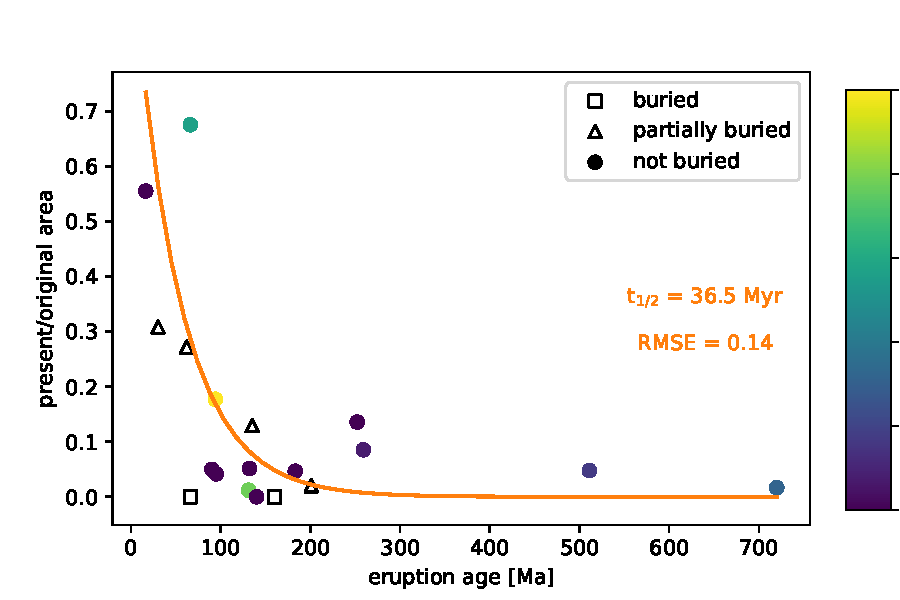
\includegraphics[width=0.6\textwidth]{Manuscript/Figures/LIP_Preservation.pdf}
	\caption{LIP preservation through time. The ratio of estimates of the present-day area to that of the original area are shown for 19 basaltic LIPs. An exponential fit is made to the 13 basaltic LIPs that have not been buried after emplacement (Table \ref{tab:LIPs}), which yields a half-life of $\sim$36~Myr. RMSE = root mean square error.}
	\label{fig:LIP_preservation}
\end{center}
\end{figure}

\begin{figure}[h!]
\begin{center}
	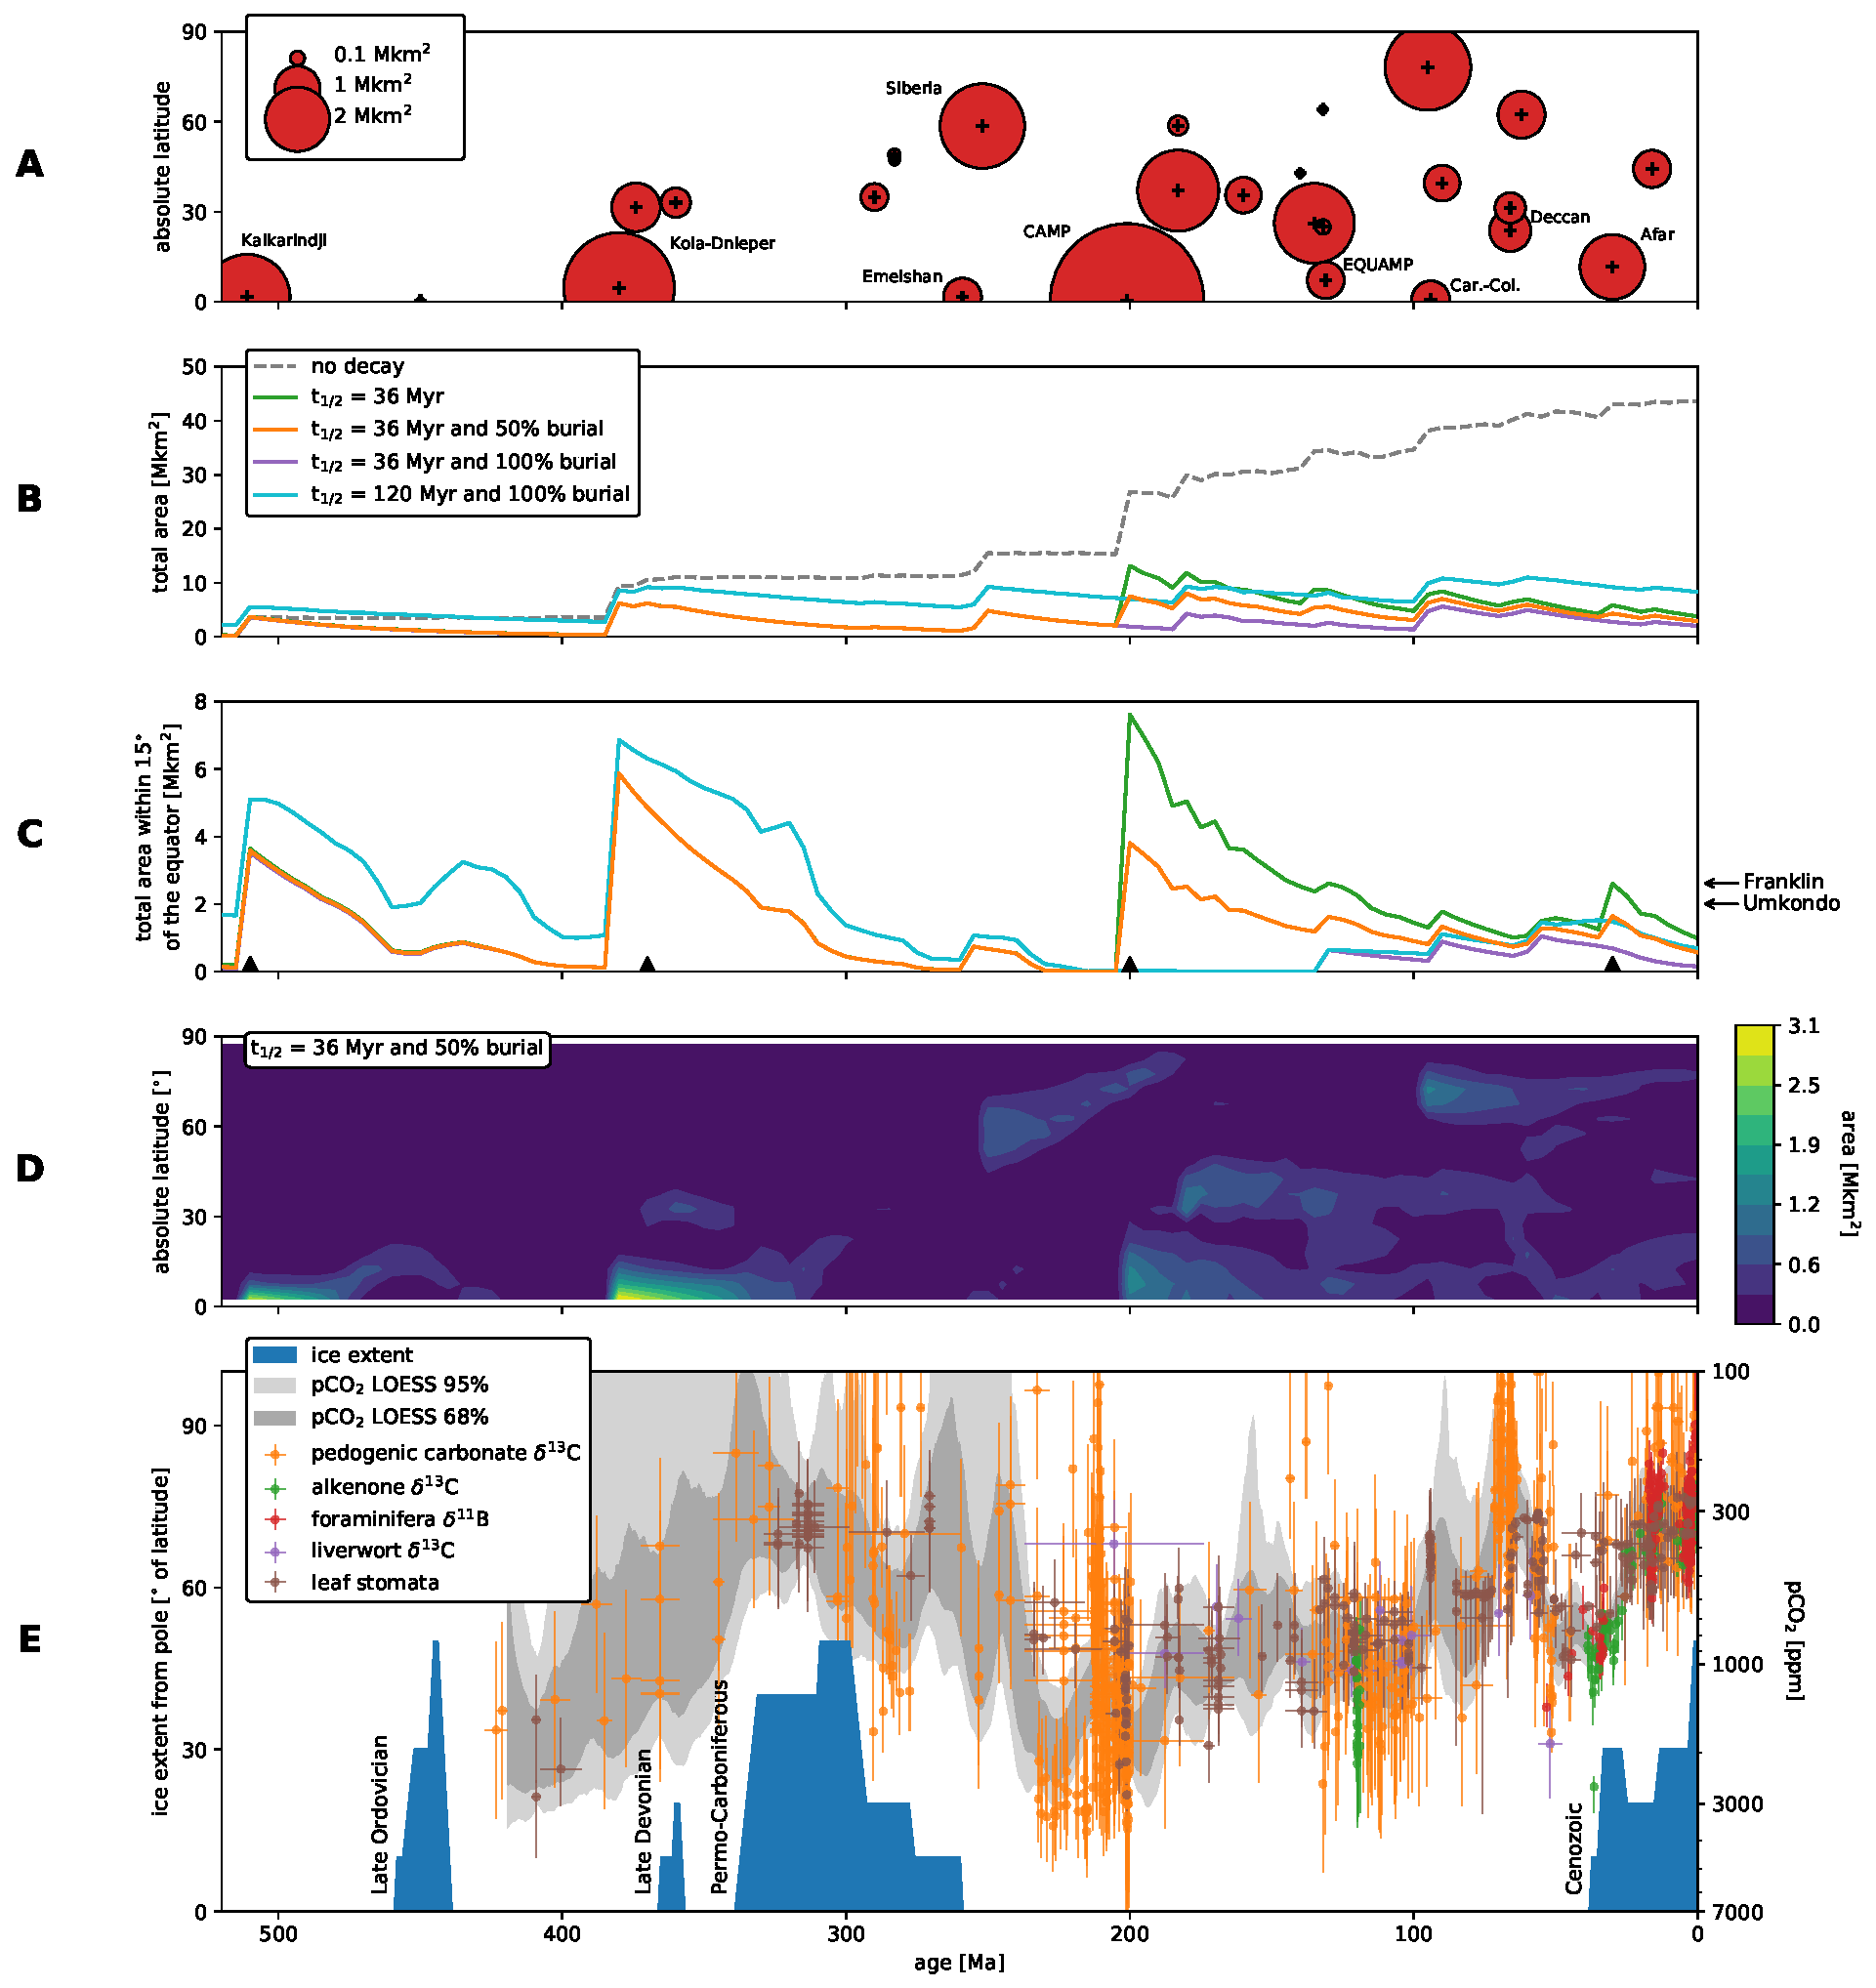
\includegraphics[width=0.8\textwidth]{Manuscript/Figures/LIP_Areas.pdf}
	\caption{\textbf{A)} LIPs included in this analysis. The size of each circle reflects the initial area estimate of each LIP. The + indicates the timing and absolute paleolatitude of the centroid of each LIP at the time of emplacement. Car.-Col. = Caribbean-Colombian. \textbf{B)} Total LIP area through time for the different post-emplacement models. Only the `no decay' model excludes pre-Phanerozoic LIPs. \textbf{C)} Tropical LIP area through time for the different post-emplacement models. The arrows to the right indicate reconstructed tropical LIP area at the time of emplacement for the ca. 720~Ma Franklin LIP and the ca. 1109~Ma Umkondo LIP. \textbf{D)} Heat map for the preferred post-emplacement model showing the latitudinal distribution of LIP area. \textbf{E)} Latitudinal extent of land ice away from the poles through time \citep{Macdonald2018a}.}
	\label{fig:LIP_area}
\end{center}
\end{figure}

\begin{figure}[h!]
\begin{center}
	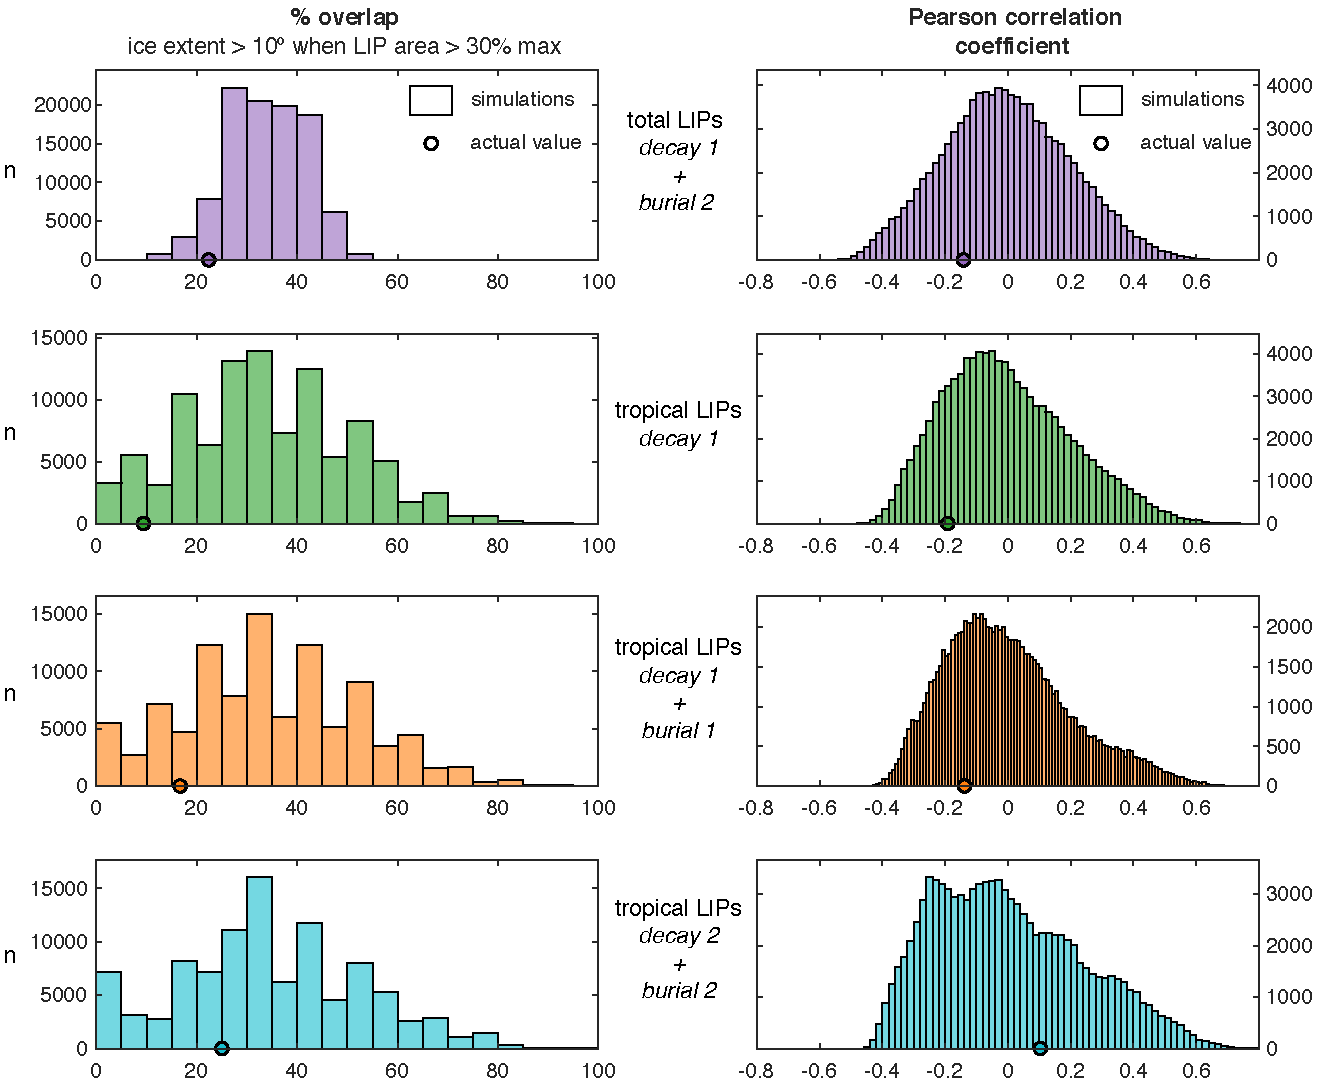
\includegraphics[width=0.85\textwidth]{Manuscript/Figures/overlap_correlation_cropped.pdf}
	\caption{The \% overlap and Pearson correlation coefficients for various LIP post-emplacement scenarios are shown with circles. These values are compared to histograms that show the range of values that arise when comparing the LIP area record to glacial intervals that have been shifted randomly in time 100,000 times.}
	\label{fig:LIP_correlation}
\end{center}
\end{figure}

\clearpage
\newpage
\footnotesize

\singlespacing

\bibliographystyle{gsabull}
\bibliography{References}

\end{document}
